\documentclass{article} % For LaTeX2e
\usepackage{nips14submit_e,times}
\usepackage{amsmath}
\usepackage{amsthm}
\usepackage{amssymb}
\usepackage{mathtools}
\usepackage{hyperref}
\usepackage{url}
\usepackage{algorithm}
\usepackage[noend]{algpseudocode}
%\documentstyle[nips14submit_09,times,art10]{article} % For LaTeX 2.09

\usepackage{mathrsfs}
\usepackage{graphicx}
\usepackage{caption}
\usepackage{subcaption}

\def\eQb#1\eQe{\begin{eqnarray*}#1\end{eqnarray*}}
\def\aB#1\aE{\begin{align*}#1\end{align*}}
\def\eQnb#1\eQne{\begin{align}#1\end{align}}
\providecommand{\e}[1]{\ensuremath{\times 10^{#1}}}
\providecommand{\pb}[0]{\pagebreak}

\newcommand{\E}{\mathrm{E}}
\newcommand{\Var}{\mathrm{Var}}
\newcommand{\Cov}{\mathrm{Cov}}

\def\Qb#1\Qe{\begin{question}#1\end{question}}
\def\Sb#1\Se{\begin{solution}#1\end{solution}}

\newenvironment{claim}[1]{\par\noindent\underline{Claim:}\space#1}{}
\newtheoremstyle{quest}{\topsep}{\topsep}{}{}{\bfseries}{}{ }{\thmname{#1}\thmnote{ #3}.}
\theoremstyle{quest}
\newtheorem*{definition}{Definition}
\newtheorem*{theorem}{Theorem}
\newtheorem*{lemma}{Lemma}
\newtheorem*{question}{Question}
\newtheorem*{preposition}{Preposition}
\newtheorem*{exercise}{Exercise}
\newtheorem*{challengeproblem}{Challenge Problem}
\newtheorem*{solution}{Solution}
\newtheorem*{remark}{Remark}
\usepackage{verbatimbox}
\usepackage{listings}
\title{Harmonic Analysis:  \\
Problem Set III}


\author{
Youngduck Choi \\
CIMS \\
New York University\\
\texttt{yc1104@nyu.edu} \\
}


% The \author macro works with any number of authors. There are two commands
% used to separate the names and addresses of multiple authors: \And and \AND.
%
% Using \And between authors leaves it to \LaTeX{} to determine where to break
% the lines. Using \AND forces a linebreak at that point. So, if \LaTeX{}
% puts 3 of 4 authors names on the first line, and the last on the second
% line, try using \AND instead of \And before the third author name.

\newcommand{\fix}{\marginpar{FIX}}
\newcommand{\new}{\marginpar{NEW}}

\nipsfinalcopy % Uncomment for camera-ready version

\begin{document}


\maketitle

\begin{abstract}
This work contains solutions to the problem set III
of Harmonic Analysis 2016 at Courant Institute of Mathematical Sciences.
\end{abstract}

\begin{question}[1]
\hfill
\begin{figure}[h!]
  \centering
    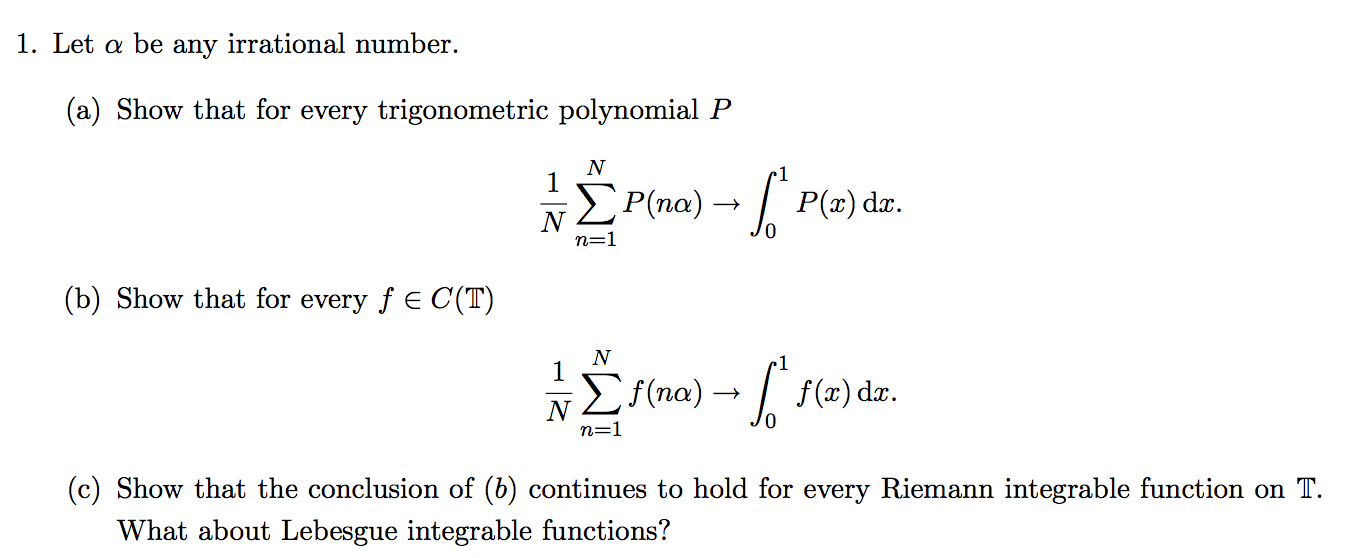
\includegraphics[width=0.8\textwidth]{HA-3-1.png}
\end{figure}
\end{question}
\begin{solution} \hfill \\
Throughout this problem, a domain of any function will be consistently defined as $\mathbb{T}$. \\
\textbf{(a)}
Let $\alpha$ be a irrational number. First, consider $e(k x)$. For $k = 0$, we have $1$ converges to $1$.
Now, for any $k \neq 0$, we have that $\int_{0}^{1} e(k x) = 0$. Furthermore, as $\alpha$ is 
an irrational, we have that $e(k \alpha ) \neq 1$. Hence, by the geometric series formula,
it follows that
\eQb
\dfrac{1}{N} \sum_{n=1}^{N} e(n\alpha ) &=& \dfrac{e(k\alpha)}{N}
\dfrac{1-e(k N \alpha )}{1-e(k\alpha)}, 
\eQe
which converges to $0$ as $N \to \infty$. Therefore, we have shown the convergence holds true
for exponentials. As trig polynomials are finite linear combinations of exponentials, 
by the linearity of limit, the convergence is true for any trig polynomial.

\bigskip

\textbf{(b)}
Fix $\epsilon > 0$. 
It follows that
By the density of trig polynomials in $C(\mathbb{T})$, there exists a polynomial $P$ such that
$||P - f||_{max} < \epsilon$. By part $(a)$, the triangle inequality, and rules of
integration, it follows that, 
\eQb
\left| \dfrac{1}{N} \sum_{n=1}^{N} f(n \alpha) - \int_{0}^{1} f(x) dx \right| 
&\leq&   
\left| \dfrac{1}{N} \sum_{n=1}^{N} f(n \alpha) 
- \dfrac{1}{N} \sum_{n=1}^{N} P(n \alpha) \right| \\
&+&  
\left| \dfrac{1}{N} \sum_{n=1}^{N} P(n \alpha)  
- \int_{0}^{1} P(x) dx \right| \\
&+& \left| \int_{0}^{1} P(x) dx  
- \int_{0}^{1} f(x) dx \right| \\ 
&\leq&   
\dfrac{1}{N} \sum_{n=1}^{N} |f(n \alpha) 
-P(n \alpha)| \\
&+&  
\left| \dfrac{1}{N} \sum_{n=1}^{N} P(n \alpha)  
- \int_{0}^{1} P(x) dx \right| \\
&+&  \int_{0}^{1} |P(x) - f(x)| dx < \epsilon + \epsilon + \epsilon = 3\epsilon, 
\eQe
for all $N$ large enough. Hence, we have shown that the convergence holds true for
all continuous functions.

\bigskip

\textbf{(c)} Before proceeding to the main part of the proof, we prove that the
asserted convergence holds true for all characteristic functions of $(a,b) \in \mathbb{T}$,
which is quite natural as the definition of Riemann integration involves a partition with
the associated upper sum and lower sum:
\begin{equation}\label{eq:convergence1}
\dfrac{1}{N} \sum_{n=1}^{N} \chi_{(a,b)}(n\alpha) \to \int_{0}^{1} 
\chi_{(a,b)}(x) dx , \> \text{ as } \> N \to \infty.
\end{equation}
Fix $\epsilon > 0$, and $(a,b) \in \mathbb{T}$. Let $f_{\epsilon}^{+}$ and $f_{\epsilon}^{-}$
be continuous functions on $\mathbb{T}$, defined by
\eQb
f_{\epsilon}^{+}(x) &=& 
\left\{
    \begin{array}{ll}
        0  & \mbox{if } x \in [0,a - \epsilon) \\
        \frac{1}{\epsilon}(x-a) + 1 & \mbox{if } x \in [a-\epsilon, a) \\   
        1 & \mbox{if } x \in [a,b) \\ 
        -\frac{1}{\epsilon}(x-b) + 1 & \mbox{if } x \in [b, b+\epsilon) \\   
        0 & \mbox{if } x \in [b + \epsilon,1], \\
    \end{array}
\right.
\eQe
and
\eQb
f_{\epsilon}^{-}(x) &=& 
\left\{
    \begin{array}{ll}
        0  & \mbox{if } x \in [0,a) \\
        \frac{1}{\epsilon}(x-a)  & \mbox{if } x \in [a , a + \epsilon) \\   
        1 & \mbox{if } x \in [a+\epsilon,b-\epsilon) \\ 
        -\frac{1}{\epsilon}(x-b)  & \mbox{if } x \in [b-\epsilon, b) \\   
        0 & \mbox{if } x \in [b,1]. \\
    \end{array}
\right.
\eQe
In particular, we have
\begin{equation} \label{eq:bound1}
b - a - 2\epsilon \leq \int_{0}^{1} f_{\epsilon}^{-}(x) dx \> \text{ and } \>
\int_{0}^{1} f_{\epsilon}^{+}(x) dx \leq b - a + 2\epsilon,
\end{equation}
along with
\begin{equation} \label{eq:bound2} 
\dfrac{1}{N} \sum_{n=1}^{N} f_{\epsilon}^{-}(n\alpha) \leq 
\dfrac{1}{N} \sum_{n=1}^{N} \chi_{(a,b)}(n\alpha) \leq
\dfrac{1}{N} \sum_{n=1}^{N} f_{\epsilon}^{+}(n\alpha). 
\end{equation} 
Now, letting $N \to \infty$ on 
both sides of \eqref{eq:bound2} respectively, we obtain
\eQb
b - a - 2\epsilon \leq \liminf_{N \to \infty} 
\dfrac{1}{N} \sum_{n=1}^{N} \chi_{(a,b)}(n\alpha) 
 \> \text{ and } 
\> \limsup_{N \to \infty}  
\dfrac{1}{N} \sum_{n=1}^{N} \chi_{(a,b)}(n\alpha)
\leq b -a + 2\epsilon. 
\eQe
As $\epsilon$ was arbitrary, we have shown that the asserted convergence is true for
all characteristic functions in $\mathbb{T}$. As before, the result can be extended
to all finite linear combinations of characteristic functions. 

\smallskip

We proceed to the main part of the proof. Fix $\epsilon > 0$. 
As $f$ is Riemann integrable, taking a fine enough partition, we have 
\eQb
\int_{0}^{1} f(x) dx - \epsilon \leq \int_{0}^{1} L_f(dx) \> \text{ and } 
\> 
\int_{0}^{1} U_f(x) dx \leq \int_{0}^{1} f(x) dx + \epsilon, 
\eQe
with 
\eQb
\dfrac{1}{N} \sum_{i=1}^{N} L_{f}(n\alpha) \leq \dfrac{1}{N} \sum_{i=1}^{N}
f(n\alpha) \leq \dfrac{1}{N} \sum_{i=1}^{N} U_{f}(n\alpha),
\eQe
where $U_f$, and $L_f$ denote the upper, lower Riemann sum of the chosen partition
respectively. In view of \eqref{eq:convergence1}, letting $N \to \infty$,  
we obtain
\eQb
\int_{0}^{1} f(x) dx - \epsilon 
\leq \liminf_{N \to \infty} 
\dfrac{1}{N} \sum_{i=1}^{N} f(n\alpha) \> \text{ and } \> 
\limsup_{N \to \infty} 
\dfrac{1}{N} \sum_{i=1}^{N} f(n\alpha) \leq 
\int_{0}^{1} f(x) dx + \epsilon.
\eQe 
As $\epsilon$ was arbitrary, we have shown that the asserted convergence is true for
all Riemann integrable functions on $\mathbb{T}$.

\smallskip

Now, for the case of Lebesgue integration, consider $\chi_{A}$, where
$A = \{ <n \alpha> \> | \> n \in \mathbb{N}\}$ ($< >$ denotes the fractional part
of a number. By definition, we have $\dfrac{1}{N}\sum_{n=1}^{N} f(n\alpha)
= 1$ for all $N$. As $A$ is countable, and $\chi_{A}$ only $1$ on measure zero set, we have that
$\int_{0}^{1}f(x)dx = 0$. Therefore, the convergence does not hold true for all Lebesgue measurable
functions.
\hfill $\qed$  

\end{solution}

\newpage

\begin{question}[2]
\hfill
\begin{figure}[h!]
  \centering
    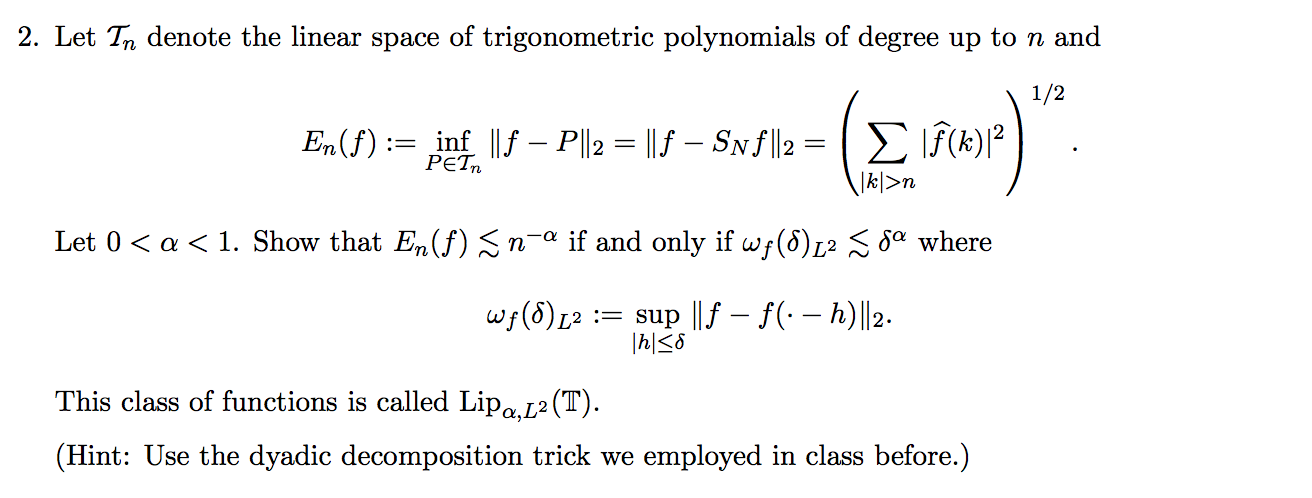
\includegraphics[width=1\textwidth]{HA-3-2.png}
\end{figure}
\end{question}
\begin{solution}
First, suppose that $\omega_{f}(\delta)_{L^2} \lesssim \delta^{\alpha}$. Using the dyadic 
decomposition trick, we have
\eQb
\sum_{k > |n|} |\hat{f}(n)|^2 \sum_{m=m_0}^{\infty}\sum_{k \in \triangle_{m}} 
\eQe
\end{solution}

\bigskip

\begin{question}[3]
\hfill
\begin{figure}[h!]
  \centering
    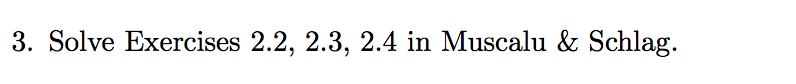
\includegraphics[width=0.5\textwidth]{HA-3-3.png}
\end{figure}
\end{question}
\begin{solution} 
\textbf{(2.2)}
We first prove the closed form formula for the Poisson Kernel. Let $0 \leq r < 1$. Then, the
Poisson Kernel is given by
\eQb
P_{r}(\theta) &=& \sum_{n \in \mathbb{Z}} r^{|n|} e(n\theta). \\
\eQe
As the series is absolutely convergent, with $\omega = re^{i\theta}$, 
by the geometric series formula, it follows that
\eQb
P_{r}(\theta) &=& \sum_{n = 0}^{\infty} \omega^n + \sum_{n=1}^{\infty} \overline{\omega}^n \\
&=& \dfrac{1}{1-\omega} + \dfrac{\overline{\omega}}{1-\overline{\omega}} 
= \dfrac{1 - |\omega|^2}{|1-\omega|^2} \\
&=& \dfrac{1-r^2}{1-2r\cos(2\pi\theta) + r^2}. 
\eQe

\bigskip

\textbf{(2.3)} Now, we show that the Poisson Kernel is an approximate identity. First, by 
the absolute convergence, we have
\eQb
\int_{\mathbb{T}} P_{r}(\theta) &=& \int_{\mathbb{T}} \sum_{n \in \mathbb{Z}}
r^{|n|}e(n\theta) 
= \sum_{n \in \mathbb{Z}} \int_{\mathbb{T}} r^{|n|}e(n\theta) 
= 1,
\eQe 
as the $n=0$ term is the only term that integrates to $1$, when all other terms 
integrates to $0$. Hence, $(A1)$ from the definition $1.3$ is verified. 
Now, observe that 
\begin{equation} \label{eq:lowcheck}
1 - 2r\cos(2\pi \theta) + r^2 = (1-r)^2 + 2r(1-\cos(2\pi\theta)).
\end{equation}
Hence, $Pr(\theta) \geq 0$ for $\theta \in \mathbb{T}$. It follows that
\eQb
\sup_{0 \leq r < 1} \int_{\mathbb{T}} |P_r(\theta)| d\theta = 1 < \infty,
\eQe
which shows that $(A2)$ is satisfied. Now, we verify the $(A3)$ property. Fix $\delta > 0$.
For $\dfrac{1}{2} \leq r \leq 1$, and $\delta \leq \theta \leq 1$, by \eqref{eq:lowcheck},
it follows that
\begin{equation}\label{eq:lowerbound1}
0 < c_{\delta} \leq 1 - 2r\cos(2\pi\theta) + r^2, 
\end{equation}
for some constant $c_{\delta}$. In view of \eqref{eq:lowerbound1}, we  obtain
\eQb
\int_{|\theta| > \delta} |P_{r}(\theta)| d\theta &\leq& 
\int_{|\theta| > \delta} \dfrac{|1-r^2|}{c_{\delta}} d\theta = \dfrac{1-\delta}{c_{\delta}}
|1-r^2|.
\eQe
Therefore, it follows that 
\eQb
\dfrac{1-\delta}{c_{\delta}} |1-r^2| \to 0 \> \text{ as } \> r \to 1^{-} \> \text{, and } \>
\int_{|\theta| > \delta} |P_{r}(\theta)| d\theta \to 0 \> \text{ as } \> r \to 1^{-},
\eQe
as required. This completes the proof that the Poisson Kernel is an approximate identity.
\bigskip

\textbf{(2.4)-(a)} From Schlag pg. 33, we have the closed form as
\eQb
Q_{r}(\theta) &=& \dfrac{2r\sin(2\pi \theta)}{1-2r\cos(2\pi \theta) + r^2}.
\eQe
As $\sin(-2\pi \theta) = -\sin(2\pi \theta)$ and $\cos(-2\pi \theta) = \cos(2\pi \theta)$,
we have 
\eQb
Q_{r}(1-\theta) &=& \dfrac{2r\sin(2\pi(1-\theta))}{1-2r\cos(2\pi (1-\theta)) + r^2} \\
&=& -\dfrac{2r\sin(2\pi \theta)}{1-2r\cos(2\pi \theta) + r^2} = -Q_{r}(\theta). 
\eQe 
Thus, $Q_r$ has an odd symmetry, centered at $\theta = 0.5$, implying that
$\int_{0}^{1} Q_r(\theta) d\theta = 0$ for all $0 < r < 1$, which violates one of the 
conditions being an approximate identity.

\bigskip

\textbf{(2.4)-(b)} By the double-angle trig identity, we have
\eQb
Q_1(\theta) &=& \dfrac{2\sin(2\pi \theta)}{2-2\cos(2\pi \theta)} 
= \dfrac{2\sin(2\pi \theta)}{2\sin^2(\pi \theta)} = \cot(\pi \theta). 
\eQe
For the graph, we have
\begin{figure}[!ht]
  \caption{A graph of $\cot(\pi \theta)$}
  \centering
    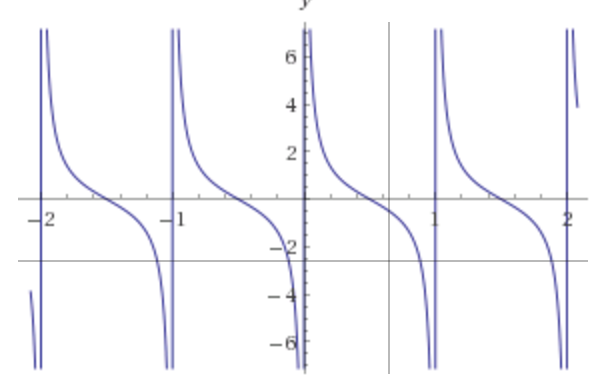
\includegraphics[width=0.5\textwidth]{cot}
\end{figure}

Now, as $\lim_{\theta \to 0} \dfrac{\sin(\theta)}{\theta} = 1$, and again using the identity,
 we have
\eQb
Q_1(\theta) = \dfrac{\cos(\pi \theta)}{\sin(\pi \theta)} 
= \dfrac{\sin(2\pi \theta)}{2\sin^2(\pi \theta)} \sim_{\theta \to 0} \dfrac{1}{\theta}, 
\> \text{ and equivalently } \> Q_1(\theta) = \Theta(\dfrac{1}{\theta}),
\eQe
as required.

\bigskip





\hfill $\qed$
\end{solution}

\bigskip

\begin{question}[4]
\hfill
\begin{figure}[h!]
  \centering
    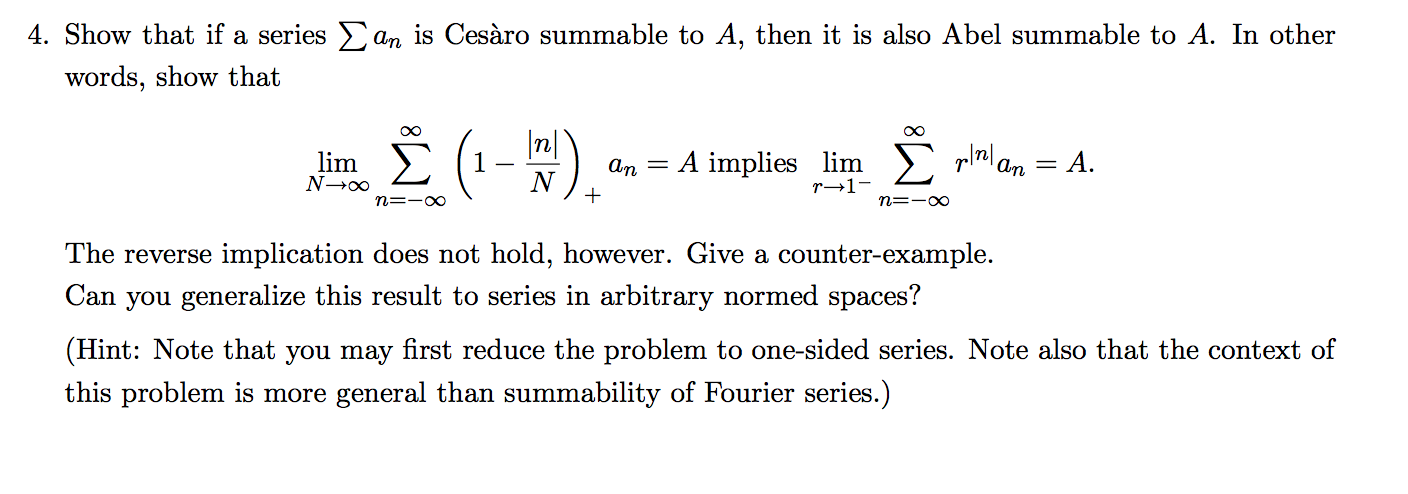
\includegraphics[width=1\textwidth]{HA-3-4.png}
\end{figure}
\end{question}
\begin{solution} \hfill \\
We first consider the case of one-sided series, with $A = 0$. Let $\sum_{n=0}^{\infty} a_n$ be
Cesaro summable to $0$. Let $s_n = \sum_{k=0}^{n} a_n$, $\sigma_n = \sum_{k=0}^{n} s_n$, and $r \in 
[0,1)$.
By Cesaro summability, we have $\sigma_n = O(n)$, and the fact that $\sum_{n=0}^{\infty}\sigma_n r^n$
converges. 
By the geometric series formula, we have
\eQb
\sum_{n=0}^{k}s_n r^n = \dfrac{1-r^{k+1}}{1-r}\sum_{n=0}^{k} a_n r^n
\eQe 
Hence, in the limit, we have the following recursive relation:
\begin{equation}\label{eq:recur1}
\sum_{n=0}^{\infty} \sigma_n r^n = (1-r)^{-1}\sum_{n=0}^{\infty} s_n r^n = (1-r)^{-2}
\sum_{n=0}^{\infty} a_n r^n,
\end{equation}
which justifies the convergence of the above series as well. 
In view of \eqref{eq:recur1}, to prove Abel summability to $0$,
it suffices to show that
\eQnb\label{eq:suffice}
\limsup_{r \to 1-} |(1-r)^2\sum_{n=0}^{\infty} \sigma_n r^n| \leq 0.
\eQne
Now, fix $\epsilon > 0$. As $ \dfrac{\sigma_n}{n+1} \to 0$, we have
\eQb
|(1-r)^2\sum_{n=0}^{\infty} \sigma_n r^n| &\leq& 
|(1-r)^2\sum_{n=0}^{N} \sigma_n r^n| + |(1-r)^2\sum_{n=N+1}^{\infty} \sigma_n r^n| \\
&\leq&
|(1-r)^2\sum_{n=0}^{N} \sigma_n r^n| + |(1-r)^2\sum_{n=N+1}^{\infty} (n+1)
\dfrac{\sigma_n}{n+1} r^n| \\
&=&
|(1-r)^2\sum_{n=0}^{N} \sigma_n r^n| + |(1-r)^2\sum_{n=N+1}^{\infty} (n+1)
r^n| \epsilon, \\
\eQe
for an $N$ large enough. As $|(1-r)^2\sum_{N+1}^{\infty} (n+1)r^n|$ is finite, and $\epsilon$ is
arbitrary, we obtain
\eQb
|(1-r)^2\sum_{n=0}^{\infty} \sigma_n r^n| &\leq&
|(1-r)^2\sum_{n=0}^{N} \sigma_n r^n| \\
\eQe
Now, with $N$ fixed, and letting $r \to 1^{-}$, we obtain \eqref{eq:suffice}.
Hence, we have shown that that $\sum_{n=0}^{\infty} a_n$ is Abel summable to $0$. 

\bigskip

Consider the series $\sum_{n=0}^{\infty} a_n$ where $a_n = (-1)^{n} n$. For every $0 \leq r < 1$, 
the Abel sum is formally given by
\eQb
A(r) &\sim& \sum_{n=0}^{\infty} (-r)^{n} n.\\
\eQe
Employing the summation by parts formula, with $a_n = n$ and $b_n = (-r)^n$, we obtain
\eQb
\sum_{n=0}^{N} n(-r)^{n} &=& N\sum_{n=0}^{N}(-r)^{n} - \sum_{n=0}^{N-1} \sum_{k=0}^{n} (-r)^{k} \\
&=& N\dfrac{1 - (-r)^{N+1}}{1+r} - \sum_{n=0}^{N-1}\dfrac{1-(-r)^{n+1}}{1+r} \\ 
&=& \dfrac{N}{1+r} - \dfrac{N(-r)^{N+1}}{1+r} - \dfrac{N-1}{1+r} + \dfrac{1}{1+r}
\sum_{n=0}^{N-1}(-r)^{n+1} \\
&=& \dfrac{1}{1+r} - \dfrac{N(-r)^{N+1}}{1+r} + \dfrac{1-(-r)^{N}}{(1+r)^2}. \\  
\eQe
Letting $N \to \infty$, we obtain
\eQb
\sum_{n=0}^{\infty}(-r)^{n}n = \dfrac{2+r}{(1+r)^2},
\eQe
and letting $r \to 1-$,
\eQb
\lim_{r \to 1-}A(r) = \dfrac{3}{4}, 
\eQe
which shows that the series considered is Abel summable. Now, we claim that
for any Cesaro summable series $\sum_{n=0}^{\infty} a_n$, we have
$\lim_{n \to \infty} \dfrac{a_n}{n} = 0$. Denote $\sigma_n$ as the
$n$th Cesaro term. Then, by basic properties of limit, it follows that
\eQb
\lim_{n \to \infty} \dfrac{a_n}{n} = \lim_{n \to \infty} \sigma_{n} - \dfrac{n-1}{n}
\sigma_{n-1} = \lim_{n \to \infty} \sigma_{n} - \lim_{n \to \infty} \dfrac{n-1}{n}
\lim_{n \to \infty} \sigma_{n-1} = 0,
\eQe 
where the last equality holds by the Cesaro summability of $\{a_n\}$. 
Observe that $\dfrac{a_n}{n} = (-1)^n$, for all $n$. Hence, the necessary condition of
Cesaro summability does not hold for the above series. Thus, the series is not Cesaro summable,
but Abel summable. We have shown that the reverse implication does not hold. 
\hfill $\qed$
\end{solution}

\bigskip


\end{document}
